\documentclass[aspectratio=1610,12pt,xcolor=dvipsnames]{beamer}
\mode<presentation>

% Respect chosen fonts (serif) and metrics
\usefonttheme{professionalfonts}
\renewcommand{\familydefault}{\rmdefault}

% Figures
\usepackage{graphicx,caption,subcaption}
\usepackage{float}

%% table
\usepackage{xcolor}
\usepackage{fancyhdr}
\usepackage{booktabs}
\usepackage[table]{xcolor}

% subsection page template
\setbeamertemplate{subsection page}
{
  \begin{centering}
    \vfill
    {\usebeamerfont{section title}\usebeamercolor[fg]{section title}\Large\insertsubsectionhead\par}
    \vfill
  \end{centering}
}
% section page template
\setbeamertemplate{section page}
{
  \begin{centering}
    \vfill
    {\usebeamerfont{section title}\usebeamercolor[fg]{section title}\Large\insertsectionhead\par}
    \vfill
  \end{centering}
}

%% footnote
\setbeamertemplate{footnote}{%
  \parindent 0em\noindent%
  \raggedright\insertfootnotemark\insertfootnotetext\par%
}

%% theme
\usetheme{default}
\useoutertheme{miniframes}
\definecolor{nagivation}{rgb}{0,0,0.35} % (typo kept if intentional)
\definecolor{main}{rgb}{0,0,0.5}
\setbeamercolor{structure}{bg=white,fg=nagivation}
\setbeamercolor{frametitle}{fg=nagivation}
\setbeamercolor{section in head/foot}{fg=white,bg=nagivation}
\setbeamertemplate{footline}[page number]
\setbeamertemplate{items}[circle]
\setbeamerfont{footnote}{size=\footnotesize}
\setbeamerfont{caption}{size=\footnotesize}
\setbeamertemplate{subsection in head/foot}{}%
\setbeamertemplate{subsection in head/foot shaded}{}%

%% font
\usepackage{dsfont}
\usepackage{newpxtext}
\usepackage{newpxmath}
\usepackage{amsmath}
\usepackage{caption}

% Math & bib
\usepackage{amsmath,amsfonts,amssymb,bm}
\DeclareMathOperator*{\argmin}{arg\,min}
\newcommand{\indep}{\perp\!\!\!\, \perp}
\usepackage{natbib}
\bibliographystyle{asr}
\setcitestyle{aysep={}}
\usepackage[english]{babel}

\makeatletter
\DeclareRobustCommand\citep
{\begingroup\scriptsize\color{gray}\NAT@swatrue\let\NAT@ctype\z@\NAT@partrue
    \@ifstar{\NAT@fulltrue\NAT@citetp}{\NAT@fullfalse\NAT@citetp}}
\makeatother

% Roman numerals macro
\newcommand{\rom}[1]{\uppercase\expandafter{\romannumeral #1\relax}}

%% Title
\title[CML]{SOC 690S: Machine Learning in Causal Inference\\[1.5pt]}
\subtitle{\large Week 3: Machine Learning Advanced\\[-10pt]}

%% author
\author[Jiang] 
{\large Wenhao Jiang\vspace{-2em}}

%% affiliation
\institute[Duke]{}
\titlegraphic{
\includegraphics[height=1.4cm]{Misc/duke_logo.png}}

\date[Duke]
{\large Department of Sociology, Fall 2025}

\begin{document}

%%%%%%%%%%%%%%%%%%%%%%%%%%%%%%%%%%%%
%%%%%%%%Begin Main Content%%%%%%%%%%
%%%%%%%%%%%%%%%%%%%%%%%%%%%%%%%%%%%%

%% Title page %%
\begin{frame}
    \titlepage 
\end{frame}

\begin{frame}{}
\vspace{-1.4em}
\setlength{\tabcolsep}{1pt}
{\footnotesize\begin{table}[h!]
\centering
\begin{tabular}{@{}llp{9.8cm}cc@{}}
\hline \hline\\[-10pt]
\textbf{\textcolor{black}{Week}} & \textbf{\textcolor{black}{Date}} & \textbf{\textcolor{black}{Topic}} & \multicolumn{2}{c@{}}{\textbf{\textcolor{black}{Problem sets}}} \\
 & & & Assign & Due \\
\hline \\[-10pt]
1  & Aug 26  & Introduction: Motivation and Linear Regression &  &  \\
2  & Sep 2  & Foundation: Machine Learning Basics &  &  \\
3  & Sep 9  & Foundation: Machine Learning Advanced & 1 &  \\
4  & Sep 16  &  Foundation: Causal Inference Basics &  &  \\
5  & Sep 23  & Foundation: Causal Inference Advanced & 2 & 1 \\[4pt]
\arrayrulecolor{gray}
\hline \\[-9pt]
6  & Sep 30  & Core: PSM and Doubly Robust Estimation & & \\
8  & Oct 7    & Core: Instrumental Variable Estimation & 3 & 2  \\
7  & Oct 14  & \textit{Fall break} &  &  \\
9  & Oct 21  & \textbf{In-class midterm} &  & \\
10  & Oct 28  &  Core: Regression Discontinuity Design &  4 & 3 \\
11  & Nov 4  & Core: Panel Data and Difference-in-Difference & & \\[4pt]
\arrayrulecolor{gray}
\hline \\[-9pt]
12  & Nov 11    & Advanced: Heterogeneous Treatment Effect & 5 & 4 \\
13 & Nov 18    & Advanced: Unstructured Data Feature Engineering & & \\
14 & Nov 25   & Advanced: Causal Reasoning in Machine Learning &  & 5 \\
 & Dec 13   & \textbf{Take-home final} & & \\
\arrayrulecolor{black}
\hline \hline
\end{tabular}
\end{table}}
\end{frame}

\section{Bias-Variance Tradeoff}

\begin{frame}
  \sectionpage
\end{frame}

\begin{frame}{Bias-Variance Tradeoff}

\begin{itemize}
    \item Any function of variables $X_i$ that approximates CEF of $Y_i$ follows the \textit{Bias-Variance Tradeoff} when evaluated using Mean Squared Error (MSE)
    \item Suppose we have a correct underlying CEF $f(\cdot)$ in the \textit{population} such that
    \begin{align*}
    Y_i &= E[Y_i \mid X_i] + \epsilon_i = f(X_i) + \epsilon_i \\
    f(x) &= E[Y_i \mid X_i=x] \\ 
    E[\epsilon_i \mid X_i=x] &= 0 \quad \textit{ CEF Decomposition Property}
    \end{align*}
\end{itemize}
\end{frame}

\begin{frame}{Bias-Variance Tradeoff}

\begin{itemize}
    \item We use a function $\hat{f}(\cdot)$ fitted using a \textit{sample} to approximate the correct \textit{population} CEF function
    \item The point-wise expected MSE at $X_i = x$, when sampled from the \textit{population} for a infinite number of times, is defined as 
    $$\textit{MSE}(x) = E\left[\left(\hat{f}(x) - f(x)\right)^2 \:\middle|\: X_i=x \right] = E\left[\left(\hat{f}(x) - f(x)\right)^2 \right]$$ \pause
    \item For any random variable $Z$ and any constant $a$
    \begin{align*}
    E\big[(Z-a)^2\big]
    &= E\big[Z^2 - 2aZ + a^2\big] \\
    &= E[Z^2] - 2aE[Z] + a^2 \\
    &= \big(E[Z^2] - (E[Z])^2\big) + \big(E[Z]-a\big)^2 \\
    &= \operatorname{Var}(Z) + \big(E[Z]-a\big)^2
\end{align*}
\end{itemize}
\end{frame}

\begin{frame}{Bias-Variance Tradeoff}

\begin{itemize}
    \item Therefore, $MSE(x)$ can be decomposed as
    \begin{align*}
    MSE(x) &= E\left[\left(\hat{f}(x) - f(x)\right)^2 \right] \\
    &= \underbrace{V\left(\hat f(x)\right)}_{\text{Variance}}
       + \underbrace{\left(E[\hat f(x)] - f(x)\right)^2}_{\text{Bias}^2}
    \end{align*}
    \item Intuitively, it means that for any approximation function based on a \textit{sample},  there is always a trade-off between the \textit{variability} of the point-wise estimate (evaluated over repeated \textit{sample} draws) and the \textit{bias} of the point-wise estimate.
\end{itemize}
\end{frame}

\begin{frame}{Tuning $\lambda$ in LASSO Regression Addresses the Tradeoff}
\begin{itemize}
    \item LASSO regression minimized the following loss function
\begin{align*}
\hat \beta_{LASSO}
&= \argmin_{b\in\mathbb{R}^{p}}
\sum_{i}^n (Y_i - X_i' b)^2
+ \lambda \cdot \sum_{j=1}^{p} |b_j|
\end{align*}
    \item At point $X_i = x$ and \textit{penalty level} $\lambda$, the prediction is given by
    \begin{align*}
        \hat f_\lambda \left(X_i = x \right) &= x' \hat\beta_{LASSO}
    \end{align*}
    \item The MSE at $X_i = x$ is then
    \begin{align*}
    \mathrm{MSE}_\lambda(x)
    = \underbrace{V\left(\hat f_\lambda(x)\right)}_{\uparrow\,\text{as }\lambda\:\downarrow}
    \;+\;
    \underbrace{\left(E\left[\hat f_\lambda(x)\right]-f(x)\right)^2}_{\downarrow\,\text{as }\lambda\:\downarrow}   
    \end{align*}
\end{itemize}
\end{frame}

\begin{frame}{Tuning $\lambda$ in LASSO Regression Addresses the Tradeoff}
\begin{itemize}
  \item Remember in $K$-fold CV, the MSE in a single fold $k$ is defined as\footnote{The MSE here has a slightly different meaning; the MSE above is relative to CEF; in the formal definition, it is relative to $Y_i$. But given the error term is stochastic, one can easily show the two essentially point to the same conclusion.}
  \begin{align*}
      MSE_{\lambda}^{k}(X_i) &= \frac{1}{m_k} \sum_{i \in B_k} \left( Y_i - \hat f^{-k}(X_i;\lambda) \right)^2 \\
      Y_i &= f(X_i) + \epsilon_i
  \end{align*}
  \item We sum up the MSE over all $x \in X_i$ in the left-out \textit{sample} $B_k$
  \item Choose \(\lambda^\ast\) by \(K\)-fold CV:
  \begin{align*}
  \lambda^\ast=\arg\min_{\lambda}\;\frac{1}{K}\sum_{k=1}^K MSE_{\lambda}^{k}(\lambda)
  \end{align*}
\end{itemize}
\end{frame}

\section{Advanced Nonlinear Machine Learning}

\begin{frame}
  \sectionpage
\end{frame}

\begin{frame}{From Linear to Non-Linear Models}

\begin{itemize}
    \item We are interested in predicting outcome $Y_i$ using regressors $X_i$, which are $p$-dimensional
    \item The \textit{best predictor} of $Y_i$ given $X_i$ is the Conditional Expectation Function
    \[
    g(X_i) = E[Y_i \mid X_i]
    \]
    \item We have used \textit{linear} prediction, such as OLS and LASSO regression, to approximate $g(X_i)$
    \item In reality, $g(X_i)$ is hardly linear, but exhibits complex non-linearities
    \item This motivates more complex models that provide more flexibilities in non-linear approximation
\end{itemize}
\end{frame}

\begin{frame}{From Linear to Non-Linear Models}

\begin{itemize}
    \item We now introduce two classes of flexible machine learning techniques
    \item Tree-based Methods and Neural Networks
    \item Both are \textit{non-linear models} that can capture complex interactions and approximations beyond linear regression
    \item Tree-based Methods and Neural Networks are commonly used as \textit{nuisance} learners inside \textit{Double Machine Learning} framework that exploit \textit{Neyman Orthogonality}
\end{itemize}
\end{frame}

\subsection{Tree-based Methods}

\begin{frame}
  \subsectionpage
\end{frame}

\begin{frame}{Tree-based Methods}

\begin{itemize}
    \item Regression trees are based on partitioning the regressor space (the space where $X_i$ takes on values) into a set of \textit{rectangles}
    \item A simple model is fit within each rectangle
    \item Since the set of splitting rules used to segment the regressor space can be summarized in a tree, these types of approaches are known as \textit{decision tree} methods
\end{itemize}
\end{frame}

\begin{frame}{Regression Trees}

\begin{itemize}
    \item The most common approach fits a simple constant model within each rectangle, which corresponds to approximating the unknown function by a \textit{step function}
    \item Given a partition into $J$ regions denoted $R_1,...,R_J$, the approximation function within each rectangle is given by
    \[
    f(X_i) = \sum_{j=1}^J \beta_j \mathds{1} (X_i \in R_j)
    \]
    where $\beta_j$ denotes a constant for each region and $\mathds{1} (\cdot)$ denotes the indicator function
\end{itemize}
\end{frame}

\begin{frame}{Regression Trees}

\begin{itemize}
    \item Suppose we have $n$ observations $(X_i,Y_i)$. The estimated coefficients for a given partition are obtained by minimizing the in-sample MSE
    \begin{align*}
        \hat \beta = \argmin_{b_1,...,b_J} \mathbb{E}\left( Y_i - \sum_{j=1}^J \beta_j \mathds{1} (x \in R_j) \right)^2
    \end{align*}
    which results in 
    \[
    \hat \beta = \text{average of } Y_i \text{ where } X_i \in R_j
    \]
\end{itemize}
\end{frame}

\begin{frame}{Regression Trees}

\begin{figure}
    \centering
  \begin{subfigure}{0.45\linewidth}
    \centering
    \raisebox{15pt}{
      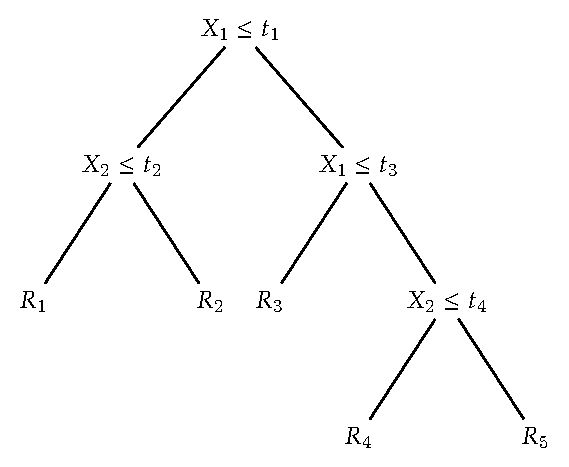
\includegraphics[width=\linewidth]{Machine Learning Advanced/Figures/step1.pdf}
    }
    \caption*{A partition tree of recursive binary splitting}
  \end{subfigure}%%
  \hspace{10pt}
  \begin{subfigure}{0.45\linewidth}
    \centering
    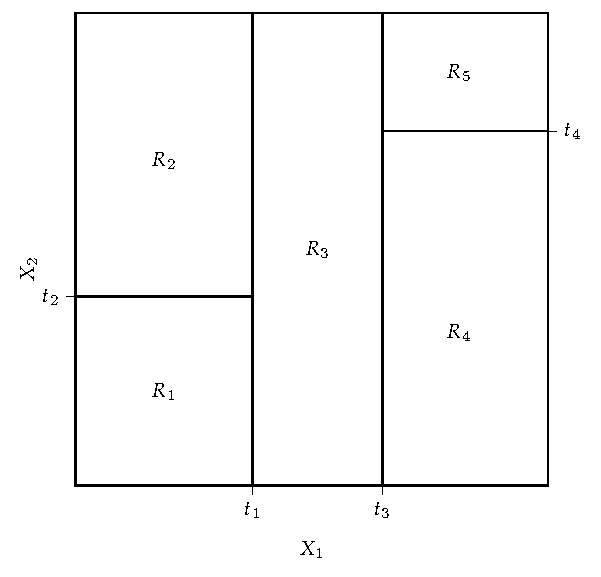
\includegraphics[width=\linewidth]{Machine Learning Advanced/Figures/step2.pdf}
    \caption*{Output of recursive binary splitting}
  \end{subfigure}
\end{figure}
\end{frame}

\begin{frame}{Regression Trees: Depth 3 Tree in Wage Prediction}

\begin{figure}
    \centering
    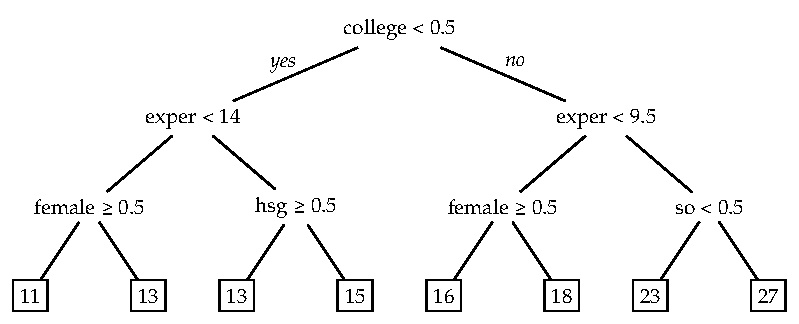
\includegraphics[width=1\linewidth]{Machine Learning Advanced/Figures/wage tree.pdf}
    \caption{Depth 3 tree in the wage prediction}
\end{figure}
\end{frame}

\begin{frame}{Growing a Regression Trees}

\begin{itemize}
    \item The key feature of trees is that the cut points for the partitions are adaptively chosen based on the data
    \item The splits are \textit{pre-specified} but are purely data dependent
    \item To make computation tractable, we use recursive binary partitioning or splitting of the regressor space
\end{itemize}
\end{frame}

\begin{frame}{Growing a Regression Tree}

\begin{itemize}
  \item At each node, consider all predictors $X_1,\dots,X_p$
  \item For each predictor $X_j$ and threshold $s$, form a binary split:
    \[
      R_L = \{i: X_{ij} \leq s\}, 
      \qquad 
      R_R = \{i: X_{ij} > s\}
    \]
  \item Compute the sum of squared errors (SSE) after the split:
    \[
      SSE(s,j) = \sum_{i \in R_L} (y_i - \bar{y}_L)^2 \;+\;
                 \sum_{i \in R_R} (y_i - \bar{y}_R)^2
    \]
    where $\bar{y}_L, \bar{y}_R$ are the mean outcomes in the two child nodes
  \item Choose $(s,j)$ that minimizes $SSE(s,j)$ (maximizes reduction in MSE)
\end{itemize}
\end{frame}

\begin{frame}{Growing a Regression Tree}

\begin{itemize}
    \item Recursively execute the procedure
    \item It is important to note that the splits in level 2 or deeper nodes may use different variables or splitting points
    \item This features analogously create ``interactions'' and ``nonlinearities'' \pause
    \item We stop growing higher-level nodes when the desired prespecified depth of the tree is reached, or (more commonly) when a prespecified minimal number of observations per region is reached
\end{itemize}
\end{frame}

\begin{frame}{Growing a Regression Tree}

\begin{itemize}
    \item Why do we care about tree depth \pause
    \item The deeper the tree grows, the smaller the bias, but the noisier (or the higher the variance) becomes, since there are fewer observations per terminal node to estimate the predicted value for this node
    \item This is the \textit{bias-variance tradeoff} at work
    \item From a prediction point of view, we can find the ``right'' depth or the structure of the tree by a validation exercise such as using a single train/test split or cross-validation (CV)
    \item The process of cutting down the branches of the tree to improve predictive performance is called \textit{tree pruning}
\end{itemize}
\end{frame}

\begin{frame}{Pruning a Tree}

\begin{itemize}
    \item It is practically not feasible to consider all possible combinations of tree structures and conduct CV
    \item A better strategy is to grow a ``full'' tree $T_0$ (that stops growing when each terminal node has fewer than some minimum number of observations) and \textit{prune} it back in order to obtain a \textit{subtree} $T$
\end{itemize}
\end{frame}

\begin{frame}{Pruning a Tree}

\begin{itemize}
    \item \textit{Cost complexity pruning}: consider a tuning penalty parameter $\lambda$, there is a \textit{subtree} $T \subset T_0$ that minimizes the in-sample MSE
    \begin{align*}
        \hat \beta = \argmin_{b_1,...,b_{|T|}} \mathbb{E}\left( Y_i - \sum_{j=1}^{b_{|T|}} \beta_j \mathds{1} (x \in R_j) \right)^2 + \lambda |T|
    \end{align*}
    where $|T|$ is the number of terminal nodes of the \textit{subtree}
    \item As in LASSO, the penalty level $\lambda$ controls the tradeoff between tree complexity and in-sample fit
    \item Optimal $\lambda$ and the corresponding tree structured is found by using either a validation set or using CV
\end{itemize}
\end{frame}

\begin{frame}{Tree-based Methods: Bagging}

    \begin{itemize}
        \item Single regression trees can still suffer from \textit{high variance} even with fine-tuning, especially when the sample size is limited
        \item \textit{Bootstrap aggregation}, or \textit{bagging} is a general-purpose procedure for reducing the variance of a statistical learning method
        \item Recall that given a set of independent variables $Z_1,...,Z_n$ each with variance $\sigma^2$, the variance of the mean $\bar Z$ is given by $\sigma^2/n$
        \item We analogously create many parallel estimates of tree-based models, and average the prediction to reduce variance
    \end{itemize}
\end{frame}

\begin{frame}{Tree-based Methods: Bagging}

    \begin{itemize}
        \item Specifically, we \textit{bootstrap} the sample for $B$ times, and construct $B$ regression trees
        \item These trees are grown deep and are \textit{not} pruned
        \item Hence each individual tree has high variance, but low bias; average these $B$ trees reduces the variance
        \item Bagging has been demonstrated to give impressive improvements in accuracy by combining together hendreds or even thoughsands of trees into a single procedure
        \[
        \hat f_{bag}(X_i) = \frac{1}{B}\sum_b \hat f^B(X_i)
        \]
    \end{itemize}
\end{frame}

\begin{frame}{Tree-based Methods: Random Forest}

\begin{itemize}
    \item \textit{Random Forests} provide an improvement over bagged trees by \textit{decorrelating} the trees
    \item As in bagging, we build a number of decision trees on bootstrapped training sample
    \item But when building these decision trees, each time a split in a tree is considered, \textit{a random sample of $m$ predictors} is chosen as split candidates from the full set of $p$ predictors
    \item A fresh sample of $m$ predictors is taken at each split, and typically we choose $m\approx \sqrt{p}$
\end{itemize}
\end{frame}

\begin{frame}{Tree-based Methods: Random Forests}

\begin{itemize}
    \item The intuition is that if there are some relatively highly-correlated predictors, one of which dominates the others in the first split, \textit{bagging} without selection of predictors is likely to produce very similar trees over bootstrapped samples
    \item Not much new information from other predictors is used with little variance reduction
    \item \textit{Random Forests} force splits to consider different subsets of predictors to reduce variance
\end{itemize}
    
\end{frame}

\begin{frame}{Tree-based Methods: Boosted Trees}

\begin{itemize}
    \item While \textit{bagged trees} and \textit{random forests} reduce variances from low-bias estimates (deep trees) through repetitive sampling, \textit{boosted trees} reduce biases from low-variance estimates (shallow trees) through recursive fitting of residuals
    \item We estimate a simple prediction rule from a shallow tree, take the \textit{residuals}, and estimate another simple shallow tree for these residuals
    \item At each step, fitting a model to the residuals from the previous step reduces the approximation error from the previous step
    \item We keep repeating this process until we reach a stopping criterion
    \item The sum of these prediction rules at each step gives the overall prediction rule
\end{itemize}
\end{frame}

\begin{frame}{Tree-based Methods: Boosted Trees}

\begin{itemize}
  \item Initialize the residuals: $R_i := Y_i, i = 1,...,n$
  \item For $j = 1,...,J$
    \begin{itemize}
      \item Fit a tree-based prediction rule $\hat{f}_j(X_i)$ to the data $(X_i, R_i)_{i=1}^n$;
      \item Update the residuals $R_i := R_i - \lambda \hat{f}_j(X_i)$, where 
            $\lambda$ is called the \textit{learning rate}
    \end{itemize}
  \item Output the boosted prediction rule
    \[
      \hat{f}(X_i) := \sum_{j=1}^J \lambda \hat{f}_j(X_i)
    \]
  \item We need make choices of tree-based prediction rule (depth), the number of learning steps $J$, and the learning rate (common default $\lambda=0.1$); these tuning parameters are typically chosen by CV
\end{itemize}
\end{frame}

\begin{frame}{Tree-based Methods: Boosted Trees}

\begin{itemize}
    \item The number of learning steps $J$ for boosting is important
    \item Since each step is building a model to predict the unexplained part of the outcome from the previous step, the in-sample prediction errors must weekly increase with each additional step
    \item If too many iterations are taken, overfitting will likely occur
    \item While too few iterations may leave significant bias in the final prediction rule
    \item In practice, the number of iterations is typically chosen by stopping the procedure once there is no marginal improvement to CV-MSE
    \item A popular implementation widely used in industry is \textit{xgboost}
\end{itemize}

\end{frame}

\subsection{Neural Networks}

\begin{frame}
  \subsectionpage
\end{frame}

\begin{frame}{Single Layer Neural Network}

\begin{itemize}
    \item A neural network takes an input vector of $p$ variables $X_i = (X_{1i}, X_{2i}, ... ,X_{pi})$ and builds a nonlinear function $f(X_i)$ to predict the response $Y_i$
    \item The $p$ features $X_{1i}, X_{2i}, ... ,X_{pi}$ make up the units in the \textit{input layer}
    \item Each of the inputs from the \textit{input layer} feeds into each of the $K$ hidden units (\textit{hidden layer})
    \item A single layer neural network has the form
    \begin{align*}
        f(X_i) &= \beta_0 + \sum_{k=1}^K \beta_k A_k = \beta_0 + \sum_{k=1}^K \beta_k h_k(X_i) \\
        &= \beta_0 + \sum_{k=1}^K \beta_k \sigma \left(w_{k0} + \sum_{j=1}^p w_{kj} X_{ji} \right)
    \end{align*}
\end{itemize}
\end{frame}

\begin{frame}{Single Layer Neural Network Visualization}

\begin{figure}
    \centering
    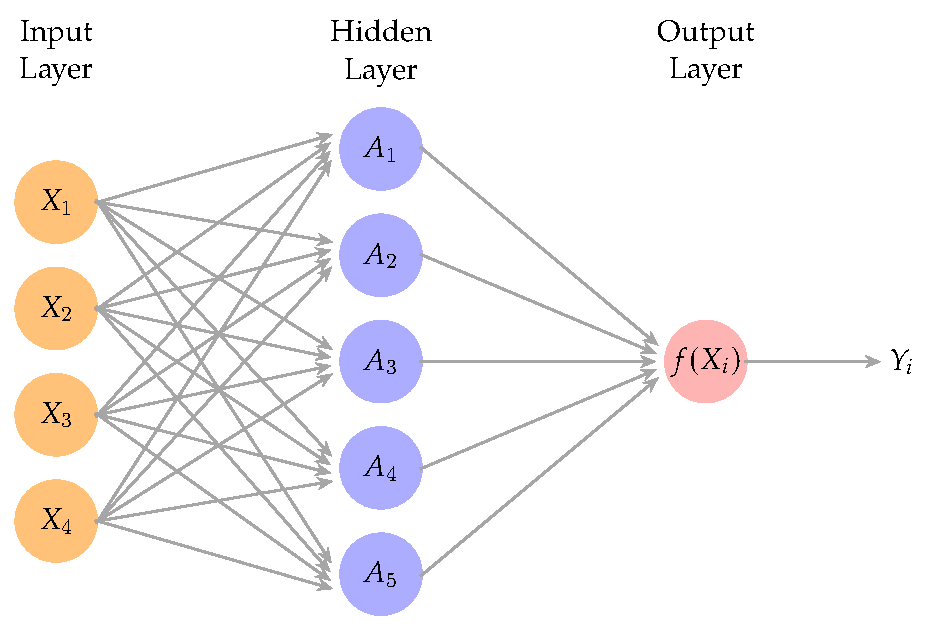
\includegraphics[width=0.7\linewidth]{Machine Learning Advanced/Figures/single layer NN.pdf}
    \caption{Neural Network with a single hidden layer}
    \label{fig:single_layer_NN}
\end{figure}
\end{frame}

\begin{frame}{Single Layer Neural Network}

\begin{itemize}
    \item There are two steps in this process
    \item First the $K$ \textit{activations} $A_k, \: k=1,...,K$, or \textit{neurons}, in the hidden layer are computed as functions of the input features $X_i,...,X_p$
    \[
    A_k = h_k(X_i) = \sigma \left( w_{k0} + \sum_{j=1}^p w_{kj} X_{ji} \right)
    \]
    \item where $\sigma(\cdot)$ is a nonlinear \textit{activation function} that is specified in advance \pause
    \item These $K$ \textit{activations} or \textit{neurons} from the hidden layer then feed into the output layer, resulting in
    \[
    f(X_i) = \beta_0 + \sum_{k=1}^{K} \beta_k A_k
    \]
    \item $\beta_k$ and $w_{kj}$ are \textit{weights}, and $\beta_0$ and $w_{k0}$ are \textit{biases}
\end{itemize}
\end{frame}

\begin{frame}{Activation Function in Neural Networks}

\begin{itemize}
    \item Popular \textit{activation functions} $\sigma(\cdot)$ include \textit{sigmoid function}
    \[
    \sigma(z) = \frac{e^z}{1+e^z} = \frac{1}{1+e^{-z}}
    \]
    \item which is the same function used in logistic regression to convert a linear function into probabilities between 0 and 1
    \end{itemize}
\end{frame}

\begin{frame}{Activation Function in Neural Networks}
    \begin{itemize}
    \item The preferred choice in modern neural networks is the \textit{ReLU} (\textit{rectified linear unit}) activation function, which takes the form
    \[
    \sigma(z) = (z)_{+} = \begin{cases}
  z & z > 0 \\[6pt]
  0 & z \leq 0
\end{cases}
    \]
    \item A \textit{ReLU} activation can be computed and stored more efficiently than a sigmoid activation; its derivative is simple
    \item Although it thresholds at 0, the constant term $w_{k0}$ shifts the inflection point
    \item Both \textit{sigmoid} and \textit{ReLU} provide the property of nonlinearity to the neural network
    \item Analogous to neurons in the brain: values in the \textit{activation function} need to exceed a threshold to be activated
\end{itemize}
\end{frame}

\begin{frame}{Nonlinear Activation Provides Nonlinear Prediction}

\begin{itemize}
    \item 2 inputs \(X=(X_1,X_2)\) and 1 hidden-layer network
    \begin{align*}
        f(X)&=\beta_0+\beta_1 h_1(X)+\beta_2 h_2(X) \\
        h_k(X)&=\sigma\big(w_{k0}+w_{k1}X_1+w_{k2}X_2\big)
    \end{align*}
    \item Now we choose a nonlinear activation \(\sigma(z)=z^2\). Other parameters are 
        \[
    \setlength{\arraycolsep}{1.5pt}
    \begin{array}{rcrcrcrcr}
      \beta_0 &=& 0, & \beta_1 &=& \frac{1}{4}, & \beta_2 &=& -\frac{1}{4} \\
      w_{10}  &=& 0, & w_{11}  &=& 1,        & w_{12} &=& 1 \\
      w_{20}  &=& 0, & w_{21}  &=& 1,        & w_{22} &=& -1
    \end{array}
    \]
    \item The \textit{hidden-layer neurons} are
    \begin{align*}
        h_1(X)=\big(0+X_1+X_2\big)^2=(X_1+X_2)^2 \\
h_2(X)=\big(0+X_1-X_2\big)^2=(X_1-X_2)^2
    \end{align*}
\end{itemize}
\end{frame}

\begin{frame}{Nonlinear Activation Provides Nonlinear Prediction}
\begin{itemize}
    \item Plugging the \textit{neurons} in the output layer 
    \begin{align*}
            f(X) &= \frac{1}{4}\left(X_1+X_2\right)^2 - \frac{1}{4}\left(X_1-X_2\right)^2 \\
    &= \frac{1}{4}\left[\left(X_1^2+2X_1X_2+X_2^2\right) - \left(X_1^2-2X_1X_2+X_2^2\right)\right] \\
    &= \frac{1}{4} \cdot 4X_1X_2 = X_1X_2
    \end{align*}
\end{itemize}
\end{frame}

\begin{frame}{Nonlinear Activation Provides Nonlinear Prediction}
    \begin{itemize}
        \item A \textit{linear} output layer on top of \textit{nonlinear} hidden units can create \textit{nonlinear functions} (here \(X_1X_2\)) even when the base model in \(X\) is linear
        \item With polynomial \(\sigma\), we recover polynomial features; with \textit{sigmoid} or \textit{ReLU}, we get flexible nonlinear combinations without being limited to fixed polynomial degree
        \item Without a nonlinear \(\sigma(\cdot)\), the network collapses to a linear model in \(X_i\) \pause
         \item Hornik, Stinchcombe, and White (1989) and Leshno et al. (1993) proved that multilayer feedforward networks are universal approximators—with a non-polynomial activation function, they can approximate any function
    \end{itemize}
\end{frame}

\begin{frame}{Number of Parameters in a Single Layer Neural Network}

\begin{itemize}
    \item In a single-layer neural network, where there are $p$ inputs and $K$ neurons, the total number of parameters to be estimated is 
    \item From \textit{input} to \textit{hidden} layer $(p+1) \times K$, or $p\times K$ \textit{weights} and $K$ \textit{biases}
    \item from \textit{hidden} to \textit{output} layer $K+1$, or $K$ \textit{weights} and $1$ \textit{bias}
    \item To minimize the loss function (suppose $Y_i$ is continuous), there are $(p+1)\times K$ \textit{weights} and $K+1$ \textit{biases} to be optimized
    \[
    \argmin_{W\in \mathbb{R}^{(p+1)\times K}; \: \beta \in \mathbb{R}^{K+1}} \sum_i \left( Y_i - f(X_i)\right)^2
    \]
\end{itemize}
\end{frame}

\begin{frame}{Multilayer Neural Network}

\begin{itemize}
    \item Single-layer networks have limited prediction power
    \item Stacking layers to multilayer neural networks can greatly improve prediction
    \item Multilayer neural networks famously solved the \textit{MNIST} handwritten-digit problem
    \begin{figure}
    \centering
    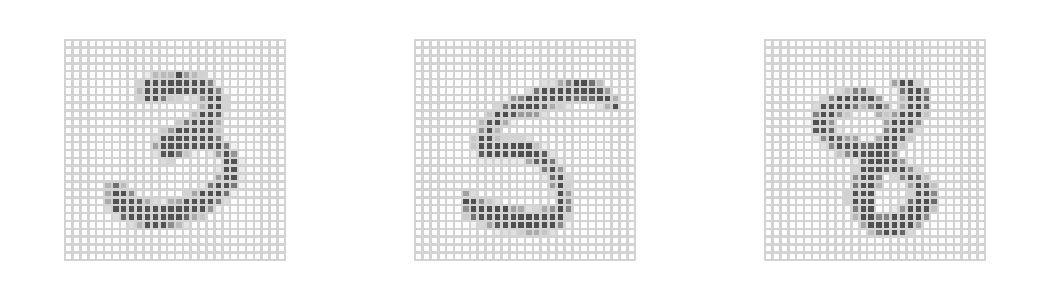
\includegraphics[width=0.65\linewidth]{Machine Learning Advanced/Figures/10_3b.pdf}
    \captionsetup{width=0.8\linewidth}
    \caption{Examples of handwritten digits from the \textit{MNIST} corpus. Each grayscale image has $28 \times 28 = 784$ pixels, each of which is an 8-bit number (0-255) which represents how dark that pixel is.}
\end{figure}
\end{itemize}
\end{frame}

\begin{frame}{Two-Layer Neural Network}

\begin{figure}
    \centering
    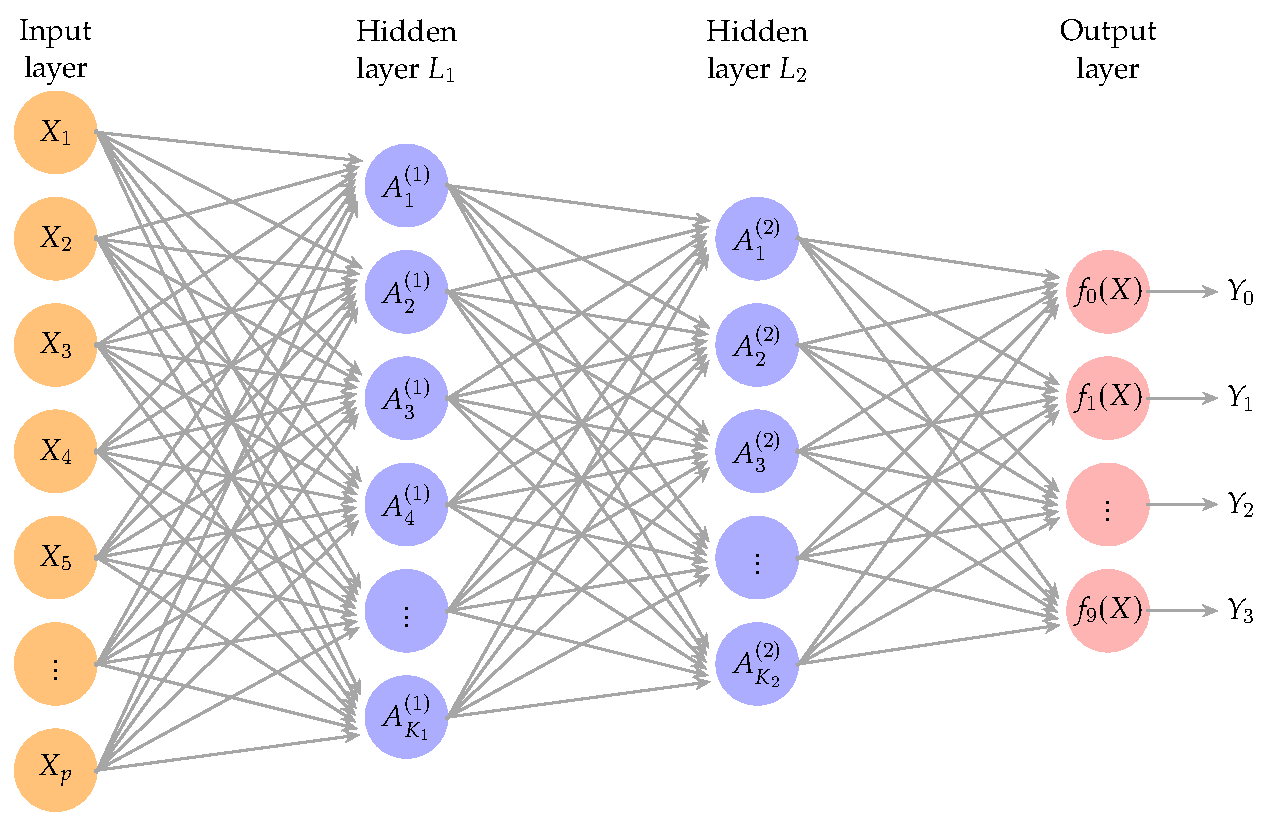
\includegraphics[width=0.8\linewidth]{Machine Learning Advanced/Figures/multilayer NN.pdf}
    \caption{Neural Network with two hidden layers and multiple outputs}
    \label{fig:multilayerNN}
\end{figure}
\end{frame}

\begin{frame}{Two-Layer Neural Network}

\begin{itemize}
    \item In the \textit{MNIST} problem, \textit{input layer} has $p = 784$ units; \textit{hidden layer} $L_1$ has $K_1=256$ units, \textit{hidden layer} $L_2$ has $K_2=128$ units, and the \textit{output layer} has 10 units corresponding to the probability that the digit is one of the 10 numbers from 0 to 9 based on a \textit{softmax} function
    \item Each \textit{neuron} $k \in 1,...,K_1$ in the first hidden layer $L_1$ is defined as
    \begin{align*}
        A_{k}^{(1)} &= h_k^{(1)}(X_i) = \sigma \left(w_{k0}^{(1)} + \sum_{j=1}^{p} w_{kj}^{(1)}X_j \right)
    \end{align*}
    \item The second hidden layer treats the \textit{neurons} $A_{k}^{(1)}$ in $L_1$ as new inputs
    \begin{align*}
        A_{\ell}^{(2)} &= h_{\ell}^{(2)}(X_i) = \sigma \left(w_{\ell 0}^{(2)} + \sum_{k=1}^{K_1} w_{\ell k}^{(2)}A_k^{(1)} \right) \quad \text{for } \ell = 1,...,K_2
    \end{align*}
\end{itemize}
\end{frame}

\begin{frame}{Number of Parameters in a Two-Layer Neural Network}

\begin{itemize}
    \item In a two-layer neural network, where there are $p$ inputs, $K_1$ neurons in the first \textit{hidden layer}, $K_2$ neurons in the second \textit{hidden layer}, and $m$ units in the \textit{output layer}, the total number of parameters to be estimated is 
    \item From \textit{input} to \textit{first hidden} layer $(p+1) \times K_1$, or $p\times K_1$ \textit{weights} and $K_1$ \textit{biases}
    \item From \textit{first hidden} to \textit{second hidden} layer $(K_1 + 1) \times K_2$, or $K_1 \times K_2$ \textit{weights} and $K_2$ \textit{biases}
    \item From \textit{second hidden} to \textit{output} layer, $(K_2+1) \times m$, or $K_2 \times m$ \textit{weights} and $m$ \textit{biases}
\end{itemize}
\end{frame}

\begin{frame}{Fitting a Neural Network}

\begin{itemize}
    \item We focus on the single layer neural network, which can be extended to multiple layers
    \item Remember to minimize the loss function (suppose $Y_i$ is continuous), there are $(p+1)\times K$ \textit{weights} and $K+1$ \textit{biases} to be optimized
    \[
    \argmin_{W\in \mathbb{R}^{(p+1)\times K}; \: \beta \in \mathbb{R}^{K+1}} \sum_i \left( Y_i - f(X_i)\right)^2
    \]
    \item This is not straightforward to minimize because
    \begin{itemize}
        \item With nonlinear \textit{activation} functions, the loss function becomes \textit{non-convex}. Gradient = 0 is necessary but no longer sufficient to find a global minimizer; we may get local minima or saddle points
        \item the sheer number of parameters makes the gradient system extremely high-dimensional and unsolvable in closed form in a single calculation
    \end{itemize}
\end{itemize}
\end{frame}

\begin{frame}{Fitting a Neural Network}

\begin{itemize}
    \item For simplicity, we represent all the parameters in one long vector $\theta$ of dimension $(p+1)K+(K+1)$
    \item Now the loss or \textit{residual} function to be minimized
    \[
    R(\theta) = \frac{1}{2} \sum_i^n \left( Y_i - f_{\theta}(X_i)\right)^2
    \]
    \item The optimal $\theta$ is derived using \textit{gradient descent} that would end up at a good \textit{local} or \textit{global} minimum
    \item Plus \textit{regularization} to penalize unimportant parameters in case of overfitting
\end{itemize}
\end{frame}

\begin{frame}{Fitting a Neural Network: Gradient Descent}

\begin{figure}
    \centering
    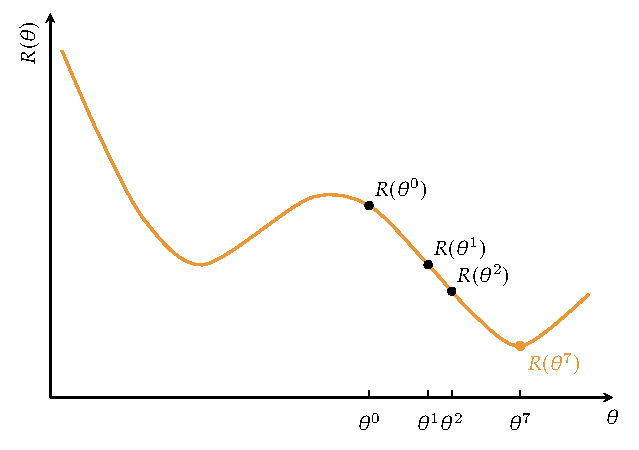
\includegraphics[width=0.63\linewidth]{Machine Learning Advanced/Figures/gradient.pdf}
    \captionsetup{width=0.9\linewidth}
    \caption{Illustration of gradient descent for one-dimensional $\theta$. The objective function $R(\theta)$ is not convex, and has two minima, one \textit{local}, the other \textit{global}}
\end{figure}
\end{frame}

\begin{frame}{Fitting a Neural Network: Gradient Descent}

\begin{itemize}
    \item We start with an initial guess of $\theta^0$ for all the parameters in $\theta$, and set $t=0$
    \item Find a vector $\delta$ that reflects a small change in $\theta$, such that $\theta^{t+1} = \theta^t + \delta$ \textit{reduces} the loss function; $R(\theta^{t+1}) < R(\theta^{t})$
    \item Stop when the improvement is negligible, \textit{e.g.},
        \[\big|R(\theta^{t+1}) - R(\theta^{t})\big| < \epsilon\] \\[-15pt] \pause
    \item $\delta$ is derived from the \textit {gradient} of $R(\theta)$ at $\theta = \theta^{t}$, where the \textit{learning rate} $\rho$ is a small positive constant
    \begin{align*}
        \delta &= -\rho \nabla R(\theta^t) \\
        &= -\rho \frac{\partial R(\theta)}{\partial \theta} \bigg|_{\theta=\theta^t}
    \end{align*}
\end{itemize}
\end{frame}

\begin{frame}{Fitting a Neural Network: Gradient Descent}

\begin{itemize}
    \item Calculating the \textit{gradient} is feasible
    \item To show this, we focus on the loss function $R_i(\theta)$ for one observation $i$; the total loss is simply the sum over the $n$ observations
    \begin{align*}
        R_i(\theta) &= \frac{1}{2} \left( Y_i - f_{\theta} (X_i) \right)^2 \\
        &= \frac{1}{2} \left( Y_i - \beta_0 \ - \sum_{k=1}^{K} \beta_k  \cdot\sigma\left(w_{k0} + \sum_{j=1}^{p} w_{kj}X_{kji} \right) \right)^2
    \end{align*}
    \item For simplicity, we write $$z_{ik} = w_{k0} + \sum_{j=1}^{p} w_{kj}X_{kji}$$
\end{itemize}
\end{frame}

\begin{frame}{Fitting a Neural Network: Gradient Descent}

\begin{itemize}
    \item For any $\beta_k$, we take the derivative with respect to $\beta_k$
    \begin{align*}
        \frac{\partial R_i(\theta)}{\partial \beta_k} &= \frac{\partial R_i(\theta)}{\partial f_{\theta}(X_i)} \cdot \frac{\partial f_{\theta}(X_i)}{\partial \beta_k} \\
        &=-(Y_i - f_{\theta}(X_i)) \cdot \sigma(z_{ik})
    \end{align*}
    \item For any $w_{kj}$, we take the derivative
    \begin{align*}
        \frac{\partial R_i(\theta)}{\partial w_{kj}} &= \frac{\partial R_i(\theta)}{\partial f_{\theta}(X_i)} \cdot \frac{\partial f_{\theta}(X_i)}{\partial \sigma(z_{ik})}  \cdot \frac{\partial \sigma(z_{ik})}{\partial z_{ik}}  \cdot \frac{\partial z_{ik}}{\partial w_{kj}} \\
        &= -(Y_i - f_{\theta}(X_i)) \cdot \beta_k \cdot \sigma'(z_{ik}) \cdot X_{kji}
    \end{align*}
    \item Notice that both expressions contain the residual $Y_i - f_{\theta}(X_i)$, meaning that the act of differentiation assigns a fraction of the target residual to each of the parameters via the chain rule—\textit{backpropagation}
\end{itemize}
\end{frame}

\begin{frame}{Fitting a Neural Network: Stochastic Gradient Descent}
    \begin{itemize}
    \item If we execute gradient descent over all $n$ observations at once, the calculation is computationally intensive
      \[
        \theta^{t+1} = \theta^t - \rho \,\frac{1}{n}\sum_{i=1}^n 
          \nabla R_i(\theta)
      \]
      \item \textit{Stochastic Gradient Descent} (SGD) instead uses only a subsample of size $B_t$ (called a \textit{mini-batch}) at each update
      \[
        \theta^{t+1} = \theta^t -\rho 
          \frac{1}{|B_t|}\sum_{i\in B_t} 
          \nabla R_i(\theta)
      \]
      \item A full pass through all observations (cycling over batches) is called an \textit{epoch}; at the beginning of each epoch, the dataset is shuffled and then split sequentially into non-overlapping \textit{mini-batches}
  \end{itemize}
\end{frame}

\begin{frame}{Fitting a Neural Network: Stochastic Gradient Descent}
  \begin{itemize}
  \item \textit{Computational efficiency:} Each update uses only a small batch of data, so updates are much faster than full-batch gradient descent
  \item \textit{Scalability:} Enables training on massive datasets that cannot fit in memory at once
  \item \textit{Online learning:} Can incorporate new observations as they arrive, without retraining from scratch
  \item \textit{Exploration of loss landscape:} The stochasticity (noise) helps the algorithm escape shallow local minima and saddle points
  \item \textit{Regularization effect:} Noisy updates often prevent overfitting, acting like an implicit form of regularization (approximately quadratic regularization similar to \textit{Ridge})
\end{itemize}
\end{frame}

\begin{frame}{Fitting a Neural Network: Dealing with Overfitting}

\begin{itemize}
    \item Just like in high-dimensional data, a massive number of parameters risks overfitting\footnote{$\sum_{j} \theta_j^2$ means we sum over the square of every scalar entry of the parameter vector $\theta$}
    \item A common $\ell_2$ Ridge penalty is used to penalize large weights or biases
      \begin{align*}
        R_i^{Ridge}(\theta) 
          &= R_i(\theta) + \lambda \sum_{j} \theta_j^2
      \end{align*}
      \item The SGD for one-observation mini-batch then updates
      \begin{align*}
          \theta^{t+1} \leftarrow \theta^t - \rho \Big( \nabla_{\theta^t} R_i(\theta^t) + 2\lambda \theta^t \Big)
      \end{align*}
\end{itemize}
\end{frame}

\begin{frame}{Fitting a Neural Network: Dealing with Overfitting}

\begin{itemize}
    \item LASSO-like regularization that filters weights are less common
    \item Instead, \textit{dropout learning} can prevent nodes from becoming over-specialized
    \begin{figure}
    \centering
  \begin{subfigure}{0.48\linewidth}
    \centering
    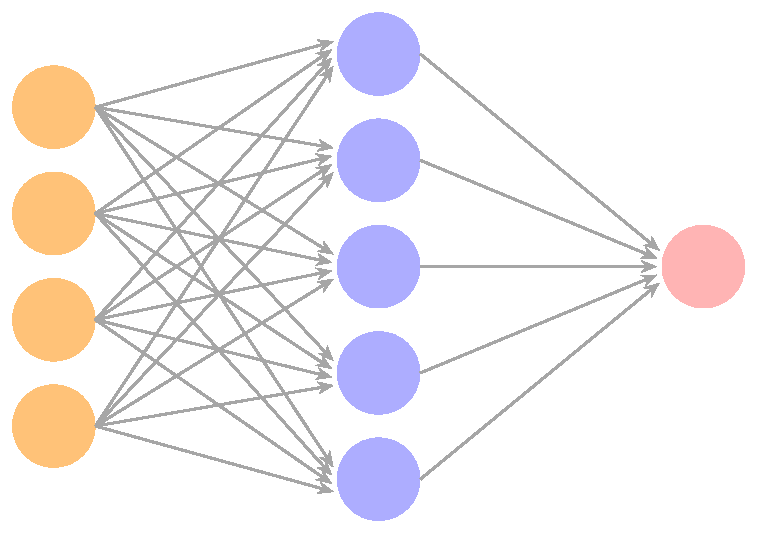
\includegraphics[width=\linewidth]{Machine Learning Advanced/Figures/dropoff1.pdf} 
    \caption*{Full Neural Network}
  \end{subfigure}%%
  \hspace{10pt}
  \begin{subfigure}{0.48\linewidth}
    \centering
    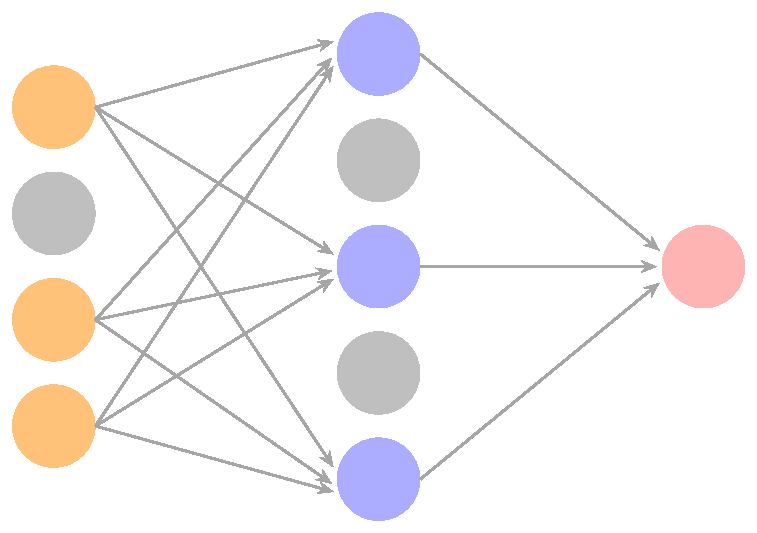
\includegraphics[width=\linewidth]{Machine Learning Advanced/Figures/dropoff2.pdf} 
    \caption*{Dropout Neural Network}
  \end{subfigure}
\end{figure}
\end{itemize}
\end{frame}

\begin{frame}{Fitting a Neural Network: Dealing with Overfitting}

\begin{itemize}
    \item In each mini-batch, a fraction $\phi$ of the units in a layer are randomly dropped (deactivated) during training
    \item The remaining units are scaled by a factor of $1/(1-\phi)$ so that the expected total input remains unchanged
    \item In practice, dropout is implemented by randomly setting the activations of the dropped units to zero, while keeping the network architecture intact
\end{itemize}

\end{frame}

\begin{frame}{Tuning a Neural Network}

There are three general classes of hyperparameters one needs to tune for neural networks to perform well

\begin{itemize}
    \item \textit{Architecture:} number of hidden layers and number of units per layer
    \item \textit{Regularization:} parameters such as $\lambda$ (weight penalty) and $\phi$ (dropout rate), which may be set separately for each layer
    \item \textit{Optimization:} details of SGD including the learning rate $\rho$, batch size, and number of epochs \pause
\end{itemize}

In practice, for neural networks (especially large ones), CV is often computationally too expensive. Instead, people use a held-out validation set and monitor performance for tuning
\end{frame}

\end{document}